\chapter{Formation des images dans les systèmes sphériques}

\section{Notion d'objet et d'image}

\ul{Le Stenope}

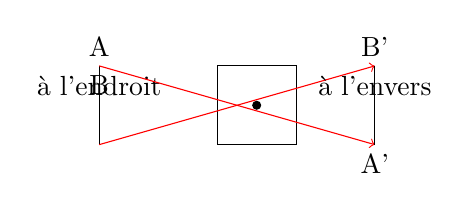
\begin{tikzpicture}
	\draw[] (-0.5, 0) rectangle (0.5, 1);
	\draw[] (-2, 0) -- (-2, 1) node [above, midway] {à l'endroit};
	\draw[red, ->] (-2, 0) -- (1.5, 1);
	\draw[red, ->] (-2, 1) -- (1.5, 0);
	\draw[] (1.5, 0) -- (1.5, 1) node [above, midway] {à l'envers};
	\draw[fill=black] (0, 0.5) circle (0.05);
	\node[above] at (-2, 1) {A};
	\node[above] at (1.5, 1) {B'};

	\node[below] at (-2, 1) {B};
	\node[below] at (1.5, 0) {A'};
\end{tikzpicture}

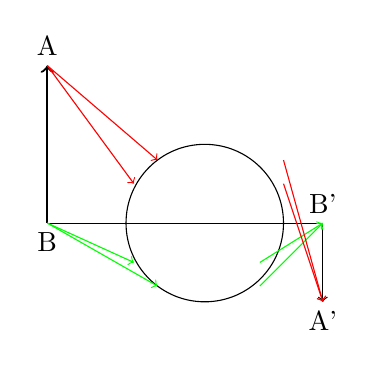
\begin{tikzpicture}

	\draw[->, thick] (0, 0) -- (0, 2);
	\draw (2, 0) circle (1);
	\draw(0, 0) -- (3.5, 0);
	\draw[->] (3.5, 0) -- (3.5, -1);
	\node[below] at (0, 0) {B};
	\node[above] at (0, 2) {A};

	\node[above] at (3.5, 0) {B'};
	\node[below] at (3.5, -1) {A'};

	\draw[->, red] (0, 2) -- (1.1, 0.5);
	\draw[->, red] (0, 2) -- (1.4, 0.8);
	\draw[->, green] (0, 0) -- (1.1, -0.5);
	\draw[->, green] (0, 0) -- (1.4, -0.8);
	
	\draw[->, green] (2.7, -0.5) -- (3.5, 0);
	\draw[->, green] (2.7, -0.8) -- (3.5, 0);

	\draw[->, red] (3, 0.5) -- (3.5, -1);
	\draw[->, red] (3, 0.8) -- (3.5, -1);
\end{tikzpicture}

Les systèmes sphériques usuelles sont : Les \ul{Lentilles minces} (convergente ou divergente) et les \ul{miroirs} (plan, concave ou convexe).

\subsection{Stigmatisme} On appel stigmatisme rigoureux, tout rayon émis par un objet ponctuel A traversant le système optique passe par \ul{Un seul point}, appelé \ul{point image A'}.

On parle de stigmatisme approché un système satisfaisant les \ul{conditions de Gauss} (utilisation de rayon très près de l'axe optique).

\subsection{Quelques définitions}
\begin{description}
	\item[Image réelle] tout rayon issu du point objet A et qui traverse le système optique passent par un point \ul{image} A'. On dit que
	\item[centré] Un système est centré s'il admet un axe de symétri de révolution (l'axe optique)
	Tout rayon arrivant suivant l'axe optique n'est pas dévié !

	\item[aplanetisme] Il y a aplanetisme si pour tout objet AB perpendiculaire sur l'axe optique on forme une image A'B' perpendiculaire par rapport à l'axe optique. En général, les systèmes optiques usuels \ul{sont aplanetique}
	\item[Centre optique] C'est le point d'intersection de l'axe optique avec le système optique. \ul{Le rayon passant par le centre optique n'est pas devie !}
\end{description}

\begin{center}
Image réelle
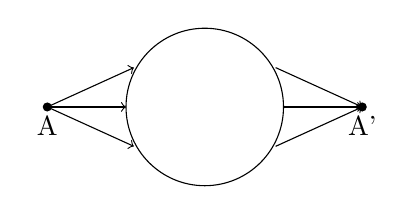
\begin{tikzpicture}
	\draw[fill=black] (0, 0) circle (0.05) node [below] {A};
	\draw[fill=black] (4, 0) circle (0.05) node [below] {A'};
	\draw (2, 0) circle (1);
	\draw[->] (0, 0) -- (1, 0);
	\draw[->] (0, 0) -- (1.1, 0.5);
	\draw[->] (0, 0) -- (1.1, -0.5);

	\draw[->] (3, 0) -- (4, 0);
	\draw[->] (2.9, 0.5) -- (4, 0);
	\draw[->] (2.9, -0.5) -- (4,0);
\end{tikzpicture}

Image virtuelles


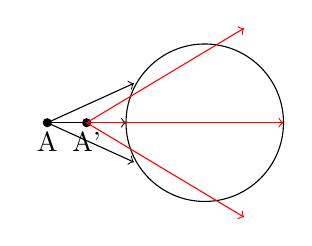
\begin{tikzpicture}
	\draw[fill=black] (0, 0) circle (0.05) node [below] {A};
	\draw[fill=black] (0.5, 0) circle (0.05) node [below] {A'};
	\draw (2, 0) circle (1);
	\draw[->] (0, 0) -- (1, 0);
	\draw[->] (0, 0) -- (1.1, 0.5);
	\draw[->] (0, 0) -- (1.1, -0.5);

	\draw[->, red] (0.5, 0) -- (2.5, 1.2);
	\draw[->, red] (0.5, 0) -- (3.0, 0.0);
	\draw[->, red] (0.5, 0) -- (2.5, -1.2);
\end{tikzpicture}
\end{center}

\section{Lentilles sphérique}

\begin{wrapfigure}[5]{r}{0pt}
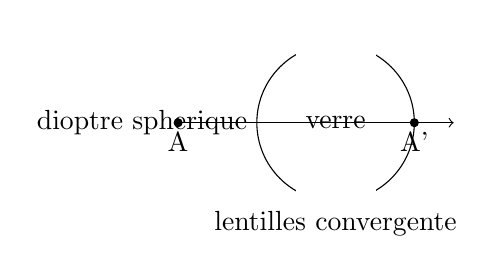
\begin{tikzpicture}
	\draw (2, 0) circle (1);
	\draw[white, fill=white] (1.5, -1.2) rectangle (2.5, 1.2);
	\node[left] at (1, 0) {dioptre spherique};
	\node at (2, 0) {verre};
	\draw[->] (0, 0) -- (3.5, 0);
	\draw[fill=black] (0, 0) circle (0.05) node [below] {A};
	\draw[fill=black] (3, 0) circle (0.05) node [below] {A'};

	\node[below] at (2, -1) {lentilles convergente};
\end{tikzpicture}
\end{wrapfigure}

On parle de lentille \ul{minces} lorsque leur epaisseur est bien plus petite que les rayons de courbures des \ul{dioptres}

~\\~\\~\\

Lentilles convergente :
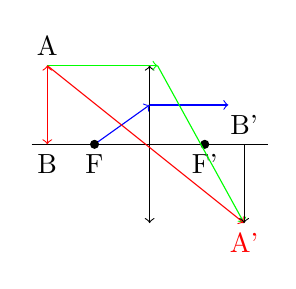
\begin{tikzpicture}
	\draw[] (0, 0) -- (3, 0);
	\draw[<->] (1.5, -1) -- (1.5, 1);
	\node[above] at (0.2, 1) {A};
	\node[below] at (0.2, 0) {B};

	\draw[<->, red] (0.2, 0) -- (0.2, 1);
	\draw[->, blue] (0.8, 0) -- (1.5, 0.5);
	\draw[->, blue] (1.5, 0.5) -- (2.5, 0.5);
	\draw[fill=black] (2.2, 0) circle (0.05) node [below] {F'};
	\draw[fill=black] (0.8, 0) circle (0.05) node [below] {F};
	\draw[green, ->] (0.2, 1) -- (1.6, 1);
	\draw[green, ->] (1.6, 1) -- (2.7, -1);
	\draw[red, ->] (0.2, 1) -- (2.7, -1) node [below] {A'};
	\draw[->] (2.7, 0) -- (2.7, -1);
	\node[above] at (2.7, 0) {B'};
\end{tikzpicture}


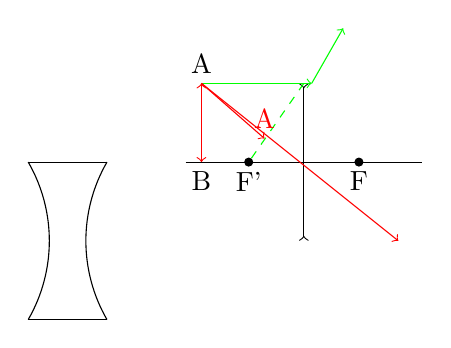
\begin{tikzpicture}
	\draw[] (-1, 0) -- (-2, 0);
	\draw[] (-1, -2) -- (-2, -2);

	\draw (-2, 0) arc (30:-30:2);
	\draw (-1, 0) arc (150:210:2);
	\draw[] (0, 0) -- (3, 0);
	\draw[>-<] (1.5, -1) -- (1.5, 1);
	\node[above] at (0.2, 1) {A};
	\node[below] at (0.2, 0) {B};

	\draw[<->, red] (0.2, 0) -- (0.2, 1);
	\draw[fill=black] (2.2, 0) circle (0.05) node [below] {F};
	\draw[fill=black] (0.8, 0) circle (0.05) node [below] {F'};

	\draw[green, ->] (0.2, 1) -- (1.6, 1);
	\draw[green, ->] (1.6, 1) -- (2, 1.7);
	\draw[green, dashed] (1.5, 1) -- (0.8, 0);
	\draw[red, ->] (0.2, 1) -- (2.7, -1);
	\draw[red, ->] (0.2, 1) -- (1, 0.3) node [above] {A};
\end{tikzpicture}

Comment trouver une image en utilisant une méthode graphique ?

Les rayons passent par le centre optique (car non dévié) et tout rayon incident parallèlent à l'axe optique passe par le \ul{foyer image F'} (après la traversé du système optique).

\ul{Le foyer objet F} : tout rayon provenant de F sort de la lentille parallèle à l'axe optique.

\ul{Plan focal image} Le plan parallèle à l'axe optique et qui passe par F'
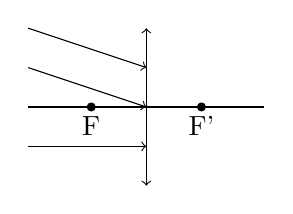
\begin{tikzpicture}
	\draw[] (0, 0) -- (3, 0);
	\draw[<->] (1.5, -1) -- (1.5, 1);
	\draw[->] (0, 1) -- (1.5, 0.5);
	\draw[->] (0, 0.5) -- (1.5, 0);
	\draw[->] (0, -0.5) -- (1.5, -0.5);

	\draw[fill=black] (2.2, 0) circle (0.05) node [below] {F'};
	\draw[fill=black] (0.8, 0) circle (0.05) node [below] {F};
\end{tikzpicture}

\paragraph{Définition} Tout rayon parallèle à une directiion donnée converge dans un point situé dans le plan image. Le rayon passant par le centre (qui n'est pas dévié) et le plan focal image.

Plan focale objet : un plan perpendiculaire par rapport à l'axe optique qui passe par le foyer objet F.

\ul{Propriété} : tout rayon provenant d'un point du plan focal objet sort parallèle à une diction donné (c'est la direction du rayon passant par ce point et par le centre optique).

\section{Formule de conjugaison}

On définit la distance focal : $f' = \overline{OF'}$

$\overline{OF} = - \overline{OF'}$

\subsection{Grandissement linéaire}

$\gamma = \frac{\overline{A'B'}}{\overline{AB}} =\frac{\overline{OA'}}{\overline{OA}}$

\subsection{Formule de conjugaison par rapport à l'axe optique}

$\frac{1}{\overline{OA'}} - \frac{1}{\overline{OA}} = \frac{1}{f'}$

\subsection{Formule de conjugaison de Newton}

$\overline{FB}*\overline{F'B'} = f^2$
